\documentclass[12pt]{article}

\usepackage{hcmus-report-template}

\setlength{\parindent}{0pt}

\renewcommand{\baselinestretch}{1.5}

\newcommand{\coursename}{Toán Ứng dụng và Thống kê}
\newcommand{\reportname}{Data Fitting và Phương Pháp OLS}
\newcommand{\reporttitle}{ĐỒ ÁN 2}

\newcommand{\studentname}{23120017 - Trần Thanh An\\23120096 - Nguyễn Viết Toàn\\23120303 - Nguyễn Hồng Ngọc\\24120278 - Võ Văn Khánh Đăng\\24120472 - Trương Huệ Trí}
\newcommand{\teachername}{Võ Nam Thục Đoan \\ Lê Nhựt Nam}

% Header
\lhead{\reporttitle}
\rhead{
Trường Đại học Khoa học Tự nhiên - ĐHQG HCM\\
\coursename
}

% Footer
\newcommand{\leftfooter}{Link Github \href{https://github.com/Coofzz/Data-Fitting-and-OLS}{Nhóm 11 - CQ2024-3}}
\lfoot{\leftfooter}

% ============ DOCUMENT ============
\begin{document}

\pagenumbering{roman}
\input{content/title.tex}

\tableofcontents
\pagebreak

\pagenumbering{arabic}
\setcounter{page}{1}

\section*{Bảng đánh giá mức độ hoàn thành và phân công công việc}
\addcontentsline{toc}{section}{Bảng đánh giá mức độ hoàn thành và phân công công việc}

\begin{table}[H]
    \centering
    \renewcommand{\arraystretch}{1.5} % Giãn dòng cho bảng dễ nhìn
    % Chỉnh lại độ rộng cột thứ 3 thành 5cm để không bị tràn viền phải
    \begin{tabular}{|c|l|p{5cm}|c|c|}
    \hline
    \textbf{MSSV} & \textbf{Họ và Tên} & \textbf{Công việc thực hiện} & \textbf{Hoàn thành} & \textbf{\% Đóng góp} \\ \hline
    23120017 & Trần Thanh An & Cài đặt phần 1 (\texttt{vif}, \texttt{ridge\_fit}, \texttt{residual\_plots}, \texttt{kfold\_cv}, Minh họa định lý Gauss–Markov) & 100\% & 25\% \\ \hline
    23120096 & Nguyễn Viết Toàn & Trưởng nhóm, Tìm dataset, tổng hợp source code và làm báo cáo & 100\% & 25\% \\ \hline
    23120303 & Nguyễn Hồng Ngọc & Không tham gia làm & 0\% & 0\% \\ \hline
    24120278 & Võ Văn Khánh Đăng & Cài đặt Phần 1 (\texttt{ols\_fit}, \texttt{hat\_matrix}, \texttt{model\_metrics}, \texttt{coef\_inference}) & 100\% & 25\% \\ \hline
    24120472 & Trương Huệ Trí & Cài đặt Phần 2  & 100\% & 25\% \\ \hline
    \end{tabular}
\end{table}
\pagebreak
\section{Phần 1: Lý Thuyết Data Fitting và Minh Họa}

% ----------------------------------------------------------
\subsection{Bài Toán Data Fitting}

\subsubsection{Phát biểu bài toán tổng quát}

Cho tập dữ liệu $\mathcal{D} = \{(\mathbf{x}_i, y_i)\}_{i=1}^{n}$ với
$\mathbf{x}_i \in \mathbb{R}^p$, $y_i \in \mathbb{R}$.
Mô hình hồi quy tuyến tính giả thiết quan hệ:
\begin{equation}
    y_i = \beta_0 + \beta_1 x_{i1} + \beta_2 x_{i2} + \cdots + \beta_p x_{ip} + \varepsilon_i
        = \mathbf{x}_i^\top \boldsymbol{\beta} + \varepsilon_i,
\end{equation}
trong đó $\boldsymbol{\beta} = (\beta_0, \beta_1, \ldots, \beta_p)^\top \in \mathbb{R}^{p+1}$
là vector tham số cần ước lượng và $\varepsilon_i$ là nhiễu ngẫu nhiên.
Dưới dạng ma trận, với ma trận design $\mathbf{X} \in \mathbb{R}^{n \times (p+1)}$
(cột đầu toàn số 1):
\begin{equation}
    \mathbf{y} = \mathbf{X}\boldsymbol{\beta} + \boldsymbol{\varepsilon}.
\end{equation}

\subsubsection{Các Giả Thiết Gauss--Markov}

\begin{itemize}
    \item \textbf{GM1 – Tuyến tính:} $\mathbf{y} = \mathbf{X}\boldsymbol{\beta} + \boldsymbol{\varepsilon}$.
    \item \textbf{GM2 – Không hoàn hảo đa cộng tuyến:} $\mathrm{rank}(\mathbf{X}) = p+1$.
    \item \textbf{GM3 – Ngoại sinh:} $\mathbb{E}[\boldsymbol{\varepsilon} \mid \mathbf{X}] = \mathbf{0}$.
    \item \textbf{GM4 – Đồng phương sai:}
        $\mathrm{Var}(\boldsymbol{\varepsilon} \mid \mathbf{X}) = \sigma^2 \mathbf{I}_n$.
    \item \textbf{GM5 – Phần dư chuẩn:}
        $\boldsymbol{\varepsilon} \mid \mathbf{X} \sim \mathcal{N}(\mathbf{0}, \sigma^2 \mathbf{I}_n)$.
\end{itemize}

% ----------------------------------------------------------
\subsection{Phương Pháp Ordinary Least Squares (OLS)}

\subsubsection{Hàm mất mát và nghiệm OLS}

Phương pháp OLS tìm $\hat{\boldsymbol{\beta}}$ tối thiểu hóa tổng bình phương phần dư
(Residual Sum of Squares -- RSS):
\begin{equation}
    \mathrm{RSS}(\boldsymbol{\beta})
    = \|\mathbf{y} - \mathbf{X}\boldsymbol{\beta}\|_2^2
    = \sum_{i=1}^{n}(y_i - \mathbf{x}_i^\top \boldsymbol{\beta})^2.
\end{equation}

\begin{theorem}[Nghiệm OLS -- Normal Equations]
Nếu $\mathbf{X}^\top\mathbf{X}$ khả nghịch, nghiệm OLS duy nhất là:
\begin{equation}
    \hat{\boldsymbol{\beta}}_{\mathrm{OLS}} = (\mathbf{X}^\top\mathbf{X})^{-1}\mathbf{X}^\top\mathbf{y}.
\end{equation}
\end{theorem}

\begin{proof}
Tính gradient của hàm mất mát theo $\boldsymbol{\beta}$:
\[
    \nabla_{\boldsymbol{\beta}}\,\mathrm{RSS} = -2\mathbf{X}^\top(\mathbf{y} - \mathbf{X}\boldsymbol{\beta}).
\]
Đặt gradient bằng không:
\[
    \mathbf{X}^\top\mathbf{X}\hat{\boldsymbol{\beta}} = \mathbf{X}^\top\mathbf{y}.
\]
Vì $\mathbf{X}^\top\mathbf{X}$ khả nghịch, nhân trái bởi $(\mathbf{X}^\top\mathbf{X})^{-1}$:
\[
    \hat{\boldsymbol{\beta}}_{\mathrm{OLS}} = (\mathbf{X}^\top\mathbf{X})^{-1}\mathbf{X}^\top\mathbf{y}.
\]
Hessian $\nabla^2_{\boldsymbol{\beta}}\,\mathrm{RSS} = 2\mathbf{X}^\top\mathbf{X}$
là ma trận xác định dương (khi $\mathrm{rank}(\mathbf{X}) = p+1$), nên nghiệm trên là
cực tiểu toàn cục duy nhất.
\end{proof}

\subsubsection{Ma Trận Chiếu và Hat Matrix}

\begin{definition}[Hat Matrix]
Ma trận chiếu (hat matrix) được định nghĩa là:
\begin{equation}
    \mathbf{H} = \mathbf{X}(\mathbf{X}^\top\mathbf{X})^{-1}\mathbf{X}^\top
              \in \mathbb{R}^{n \times n}.
\end{equation}
Tên gọi xuất phát từ việc $\mathbf{H}$ ``đội mũ'' lên $\mathbf{y}$:
$\hat{\mathbf{y}} = \mathbf{H}\mathbf{y}$.
\end{definition}

\noindent\textbf{Các tính chất của $\mathbf{H}$:}
\begin{enumerate}
    \item \textit{Idempotent:} $\mathbf{H}^2 = \mathbf{H}$.
    \item \textit{Đối xứng:} $\mathbf{H}^\top = \mathbf{H}$.
    \item Giá trị riêng chỉ là $0$ hoặc $1$.
    \item $\mathrm{rank}(\mathbf{H}) = p+1$.
    \item Phần dư: $\hat{\boldsymbol{\varepsilon}} = (\mathbf{I} - \mathbf{H})\mathbf{y}$.
\end{enumerate}

\begin{proof}[Chứng minh $\mathbf{H}^2 = \mathbf{H}$]
\[
    \mathbf{H}^2
    = \bigl[\mathbf{X}(\mathbf{X}^\top\mathbf{X})^{-1}\mathbf{X}^\top\bigr]
      \bigl[\mathbf{X}(\mathbf{X}^\top\mathbf{X})^{-1}\mathbf{X}^\top\bigr]
    = \mathbf{X}(\mathbf{X}^\top\mathbf{X})^{-1}
      \underbrace{[\mathbf{X}^\top\mathbf{X}](\mathbf{X}^\top\mathbf{X})^{-1}}_{=\mathbf{I}}
      \mathbf{X}^\top
    = \mathbf{H}. \qedhere
\]
\end{proof}

\subsubsection{Định Lý Gauss--Markov}

\begin{theorem}[Gauss--Markov -- BLUE]
Dưới các giả thiết GM1--GM4:
\begin{enumerate}
    \item \textbf{Không chệch:} $\mathbb{E}[\hat{\boldsymbol{\beta}}_{\mathrm{OLS}} \mid \mathbf{X}] = \boldsymbol{\beta}$.
    \item \textbf{Ma trận hiệp phương sai:}
        $\mathrm{Var}(\hat{\boldsymbol{\beta}}_{\mathrm{OLS}} \mid \mathbf{X}) = \sigma^2(\mathbf{X}^\top\mathbf{X})^{-1}$.
    \item \textbf{BLUE:} Trong lớp các ước lượng tuyến tính không chệch,
        OLS có phương sai nhỏ nhất.
\end{enumerate}
\end{theorem}

\subsubsection{Ước Lượng Phương Sai Nhiễu}

Sau khi có $\hat{\boldsymbol{\beta}}_{\mathrm{OLS}}$, ước lượng không chệch của
$\sigma^2$ là:
\begin{equation}
    \hat{\sigma}^2 = \frac{\mathrm{RSS}}{n - p - 1}
                   = \frac{\|\mathbf{y} - \mathbf{X}\hat{\boldsymbol{\beta}}\|^2}{n - p - 1}.
\end{equation}
Ta chia cho $(n-p-1)$ vì đã ước lượng $(p+1)$ tham số, làm mất đi $(p+1)$ bậc tự do.
Có thể chứng minh $\mathbb{E}[\hat{\sigma}^2] = \sigma^2$.

% ----------------------------------------------------------
\subsection{Đánh Giá Mô Hình}

\subsubsection{Phân rã tổng bình phương}

Gọi $\bar{y} = \frac{1}{n}\sum y_i$. Ta có phân rã:
\begin{equation}
    \underbrace{\sum(y_i - \bar{y})^2}_{\mathrm{TSS}}
    = \underbrace{\sum(\hat{y}_i - \bar{y})^2}_{\mathrm{ESS}}
    + \underbrace{\sum(y_i - \hat{y}_i)^2}_{\mathrm{RSS}}.
\end{equation}

\subsubsection{Hệ số xác định $R^2$ và $\bar{R}^2$}

\begin{equation}
    R^2 = 1 - \frac{\mathrm{RSS}}{\mathrm{TSS}} = \frac{\mathrm{ESS}}{\mathrm{TSS}} \in [0,1].
\end{equation}
$R^2$ không bao giờ giảm khi thêm biến. Để so sánh mô hình với số biến khác nhau, ta dùng
$R^2$ hiệu chỉnh:
\begin{equation}
    \bar{R}^2 = 1 - \frac{n-1}{n-p-1}(1 - R^2).
\end{equation}

\subsubsection{Kiểm Định Giả Thuyết}

\paragraph{Kiểm định $t$ (Student's $t$-test).}
Giả thuyết $H_0: \beta_j = 0$ (biến $X_j$ không có ý nghĩa trong mô hình).
Dưới GM5, $\hat{\boldsymbol{\beta}}_{\mathrm{OLS}} \mid \mathbf{X} \sim
\mathcal{N}(\boldsymbol{\beta},\, \sigma^2(\mathbf{X}^\top\mathbf{X})^{-1})$.
Thống kê kiểm định:
\begin{equation}
    t_j = \frac{\hat{\beta}_j}{\mathrm{SE}(\hat{\beta}_j)} \sim t_{n-p-1}
    \quad \text{(dưới } H_0\text{)},
\end{equation}
với $\mathrm{SE}(\hat{\beta}_j) = \hat{\sigma}\sqrt{[(\mathbf{X}^\top\mathbf{X})^{-1}]_{jj}}$.
Khoảng tin cậy 95\%:
\begin{equation}
    \mathrm{CI}_{95}(\beta_j) =
    \bigl[\hat{\beta}_j - t_{\alpha/2,\,n-p-1} \cdot \mathrm{SE}(\hat{\beta}_j),\;
          \hat{\beta}_j + t_{\alpha/2,\,n-p-1} \cdot \mathrm{SE}(\hat{\beta}_j)\bigr].
\end{equation}

\paragraph{Kiểm định $F$ cho mô hình tổng thể.}
$H_0: \beta_1 = \beta_2 = \cdots = \beta_p = 0$.
\begin{equation}
    F = \frac{(\mathrm{TSS} - \mathrm{RSS})/p}{\mathrm{RSS}/(n-p-1)} \sim F_{p,\,n-p-1}.
\end{equation}

% ----------------------------------------------------------
\subsection{Các Vấn Đề Nâng Cao trong Data Fitting}

\subsubsection{Đa cộng tuyến (Multicollinearity)}

Đa cộng tuyến xảy ra khi các cột của $\mathbf{X}$ có tương quan cao, khiến
$\mathbf{X}^\top\mathbf{X}$ gần suy biến. Hệ số phóng đại phương sai (VIF):
\begin{equation}
    \mathrm{VIF}_j = \frac{1}{1 - R_j^2},
\end{equation}
trong đó $R_j^2$ là $R^2$ khi hồi quy biến $X_j$ theo các biến còn lại.
VIF $> 10$ cho thấy đa cộng tuyến nghiêm trọng.

\subsubsection{Hồi Quy Ridge và Lasso (Regularization)}

\textbf{Ridge Regression (L2):}
\begin{equation}
    \hat{\boldsymbol{\beta}}_{\mathrm{ridge}}
    = \arg\min_{\boldsymbol{\beta}}
      \bigl\{\|\mathbf{y} - \mathbf{X}\boldsymbol{\beta}\|^2 + \lambda\|\boldsymbol{\beta}\|_2^2\bigr\}
    = (\mathbf{X}^\top\mathbf{X} + \lambda\mathbf{I})^{-1}\mathbf{X}^\top\mathbf{y}.
\end{equation}

\textbf{Lasso Regression (L1):}
\begin{equation}
    \hat{\boldsymbol{\beta}}_{\mathrm{lasso}}
    = \arg\min_{\boldsymbol{\beta}}
      \bigl\{\|\mathbf{y} - \mathbf{X}\boldsymbol{\beta}\|^2 + \lambda\|\boldsymbol{\beta}\|_1\bigr\}.
\end{equation}
Lasso không có nghiệm closed-form; giải bằng coordinate descent hoặc subgradient methods.

\subsubsection{Phân Tích Phần Dư (Residual Analysis)}

Bốn biểu đồ chẩn đoán chuẩn mực:
\begin{enumerate}
    \item \textbf{Residuals vs Fitted:} Kiểm tra tính tuyến tính và đồng phương sai.
    \item \textbf{Normal Q-Q:} Kiểm tra tính chuẩn của phần dư.
    \item \textbf{Scale-Location:} Kiểm tra homoscedasticity.
    \item \textbf{Cook's Distance:} Xác định các quan sát ảnh hưởng lớn.
        Công thức: $D_i = \dfrac{r_i^2}{p} \cdot \dfrac{h_{ii}}{1 - h_{ii}}$,
        với $h_{ii}$ là đường chéo của $\mathbf{H}$, $r_i$ là phần dư chuẩn hóa.
\end{enumerate}

\subsubsection{Cross-Validation và Lựa Chọn Mô Hình}

$k$-Fold Cross-Validation:
\begin{equation}
    \mathrm{CV}(k) = \frac{1}{k}\sum_{i=1}^{k}\mathrm{MSE}_i.
\end{equation}
Tiêu chí lựa chọn mô hình:
\begin{equation}
    \mathrm{AIC} = n\ln\!\left(\frac{\mathrm{RSS}}{n}\right) + 2(p+2), \qquad
    \mathrm{BIC} = n\ln\!\left(\frac{\mathrm{RSS}}{n}\right) + (p+2)\ln n.
\end{equation}

% ----------------------------------------------------------
\subsection{Hàm \texttt{ols\_fit(X, y)}}

\subsubsection{Cơ sở Lý thuyết \& Công thức Toán học}

Hàm \texttt{ols\_fit} ước lượng hệ số hồi quy OLS theo công thức
$\hat{\boldsymbol{\beta}} = (\mathbf{X}^\top\mathbf{X})^{-1}\mathbf{X}^\top\mathbf{y}$
và tính phương sai nhiễu $\hat{\sigma}^2 = \mathrm{RSS}/(n-p-1)$.
Các hàm ma trận hỗ trợ được cài đặt từ đầu gồm:
\texttt{mat\_zeros}, \texttt{mat\_transpose}, \texttt{mat\_mul},
\texttt{mat\_vec\_mul}, \texttt{mat\_inverse}, \texttt{mat\_identity},
\texttt{add\_intercept}.

\subsubsection{Kết quả Cài đặt \& Kiểm chứng}

Hàm trả về dictionary gồm: \texttt{beta\_hat}, \texttt{sigma2}, \texttt{rss},
\texttt{y\_hat}, \texttt{residuals}, \texttt{n}, \texttt{p}, \texttt{dof}.
Năm unit test được chạy và so sánh với \texttt{numpy.linalg.lstsq}. Ở đây kiểm tra cả 3 hàm \texttt{ols\_fit}, \texttt{hat\_matrix}, \texttt{model\_metrics} tại đây, do 3 hàm đều có input giống nhau, nên thực hiện 5 unit test chung input.

\begin{itemize}
    \item \textbf{Unit Test 1:} $y = -1.5 + 1.5x$, dữ liệu 6 điểm.
    \item \textbf{Unit Test 2:} $y = 2 + 3x$, dữ liệu 5 điểm (fit hoàn hảo).
    \item \textbf{Unit Test 3:} $y = 2x$ (không intercept), 4 điểm.
    \item \textbf{Unit Test 4:} $y = 1 + 2x_1 + 0.5x_2$, hồi quy bội 6 điểm.
    \item \textbf{Unit Test 5:} $y \approx 2x$, dữ liệu có nhiễu, 6 điểm.
\end{itemize}

\begin{figure}[H]
    \centering
    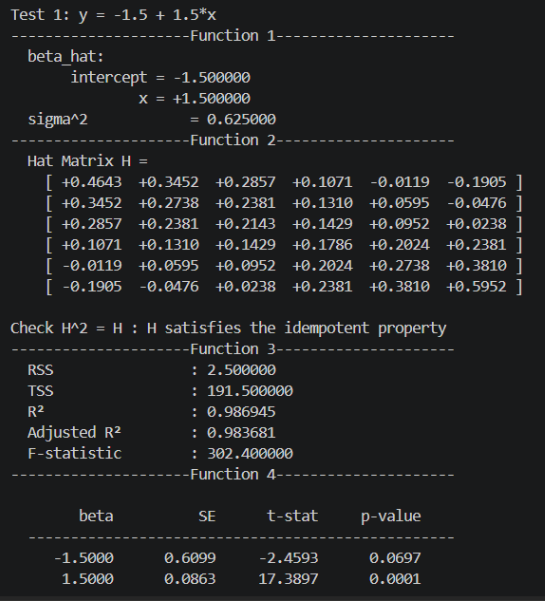
\includegraphics[width=0.85\textwidth]{images/part1/fig_test1_output.png}
    \caption{Kết quả Unit Test 1: $y = -1.5 + 1.5x$.
             Hàm \texttt{ols\_fit} cho $\hat{\beta}_0 = -1.5$, $\hat{\beta}_1 = 1.5$,
             $\hat{\sigma}^2 = 0.625$.}
    \label{fig:test1_output}
\end{figure}

\begin{figure}[H]
    \centering
    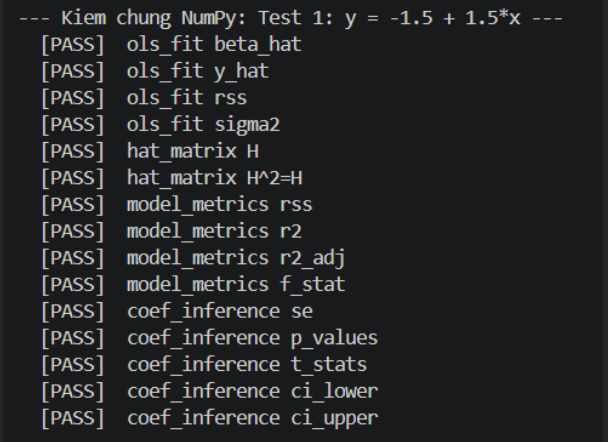
\includegraphics[width=0.75\textwidth]{images/part1/fig_test1_verify.png}
    \caption{Kiểm chứng NumPy -- Test 1: tất cả các mục đều \texttt{[PASS]}.}
    \label{fig:test1_verify}
\end{figure}

\begin{figure}[H]
    \centering
    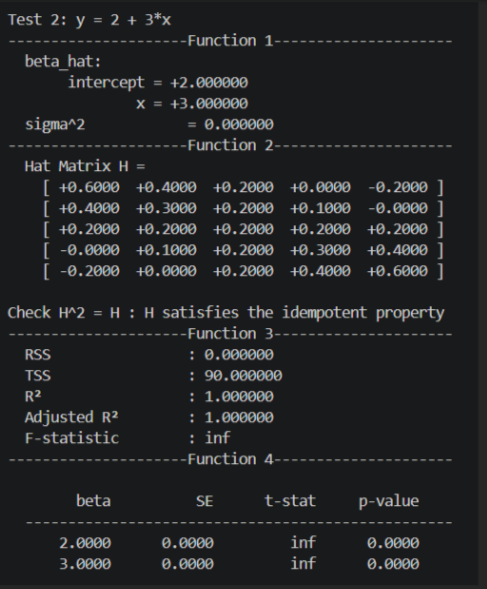
\includegraphics[width=0.85\textwidth]{images/part1/fig_test2_output.png}
    \caption{Kết quả Unit Test 2: $y = 2 + 3x$ (fit hoàn hảo, $\hat{\sigma}^2 = 0$,
             $R^2 = 1$, $F\text{-stat} = \infty$).}
    \label{fig:test2_output}
\end{figure}

\begin{figure}[H]
    \centering
    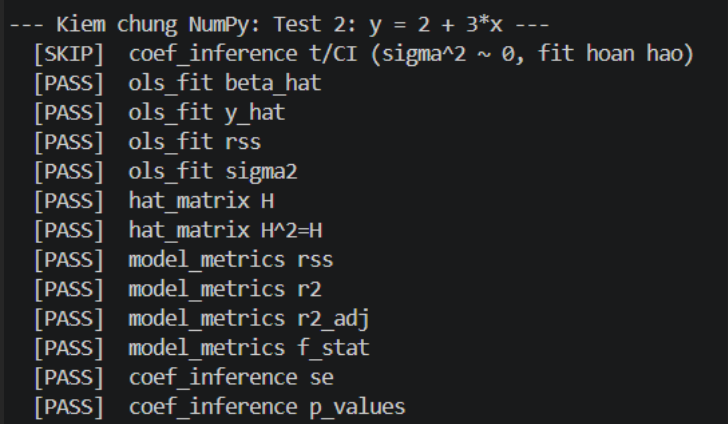
\includegraphics[width=0.75\textwidth]{images/part1/fig_test2_verify.png}
    \caption{Kiểm chứng NumPy -- Test 2: tất cả các mục \texttt{[PASS]}.}
    \label{fig:test2_verify}
\end{figure}

\begin{figure}[H]
    \centering
    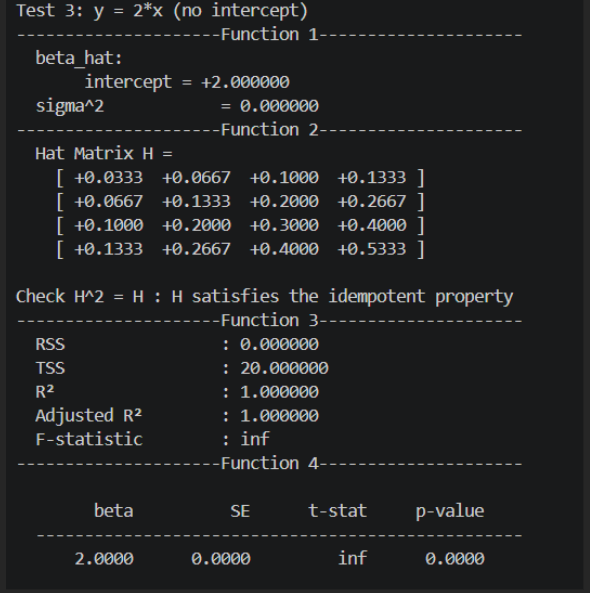
\includegraphics[width=0.85\textwidth]{images/part1/fig_test3_output.png}
    \caption{Kết quả Unit Test 3: $y = 2x$ (không intercept, fit hoàn hảo).}
    \label{fig:test3_output}
\end{figure}

\begin{figure}[H]
    \centering
    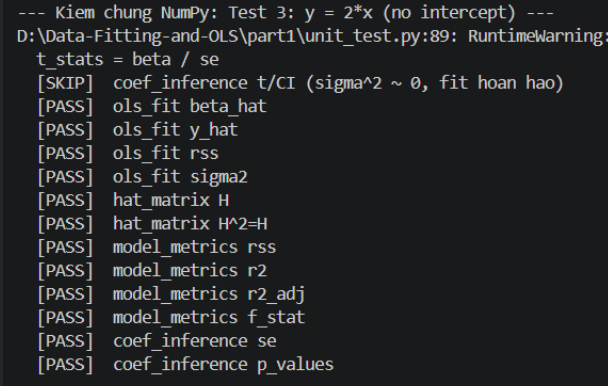
\includegraphics[width=0.75\textwidth]{images/part1/fig_test3_verify.png}
    \caption{Kiểm chứng NumPy -- Test 3.}
    \label{fig:test3_verify}
\end{figure}

\begin{figure}[H]
    \centering
    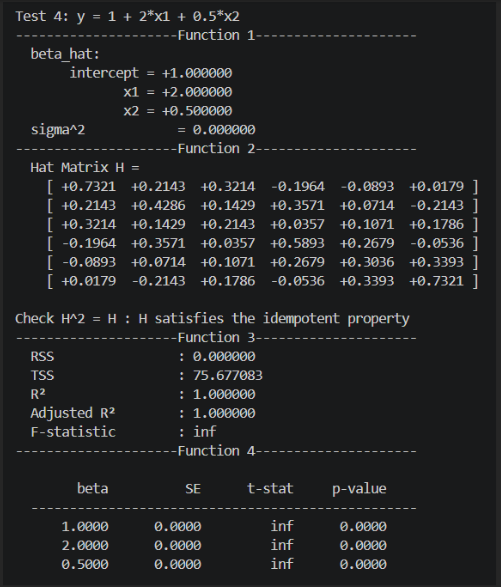
\includegraphics[width=0.85\textwidth]{images/part1/fig_test4_output.png}
    \caption{Kết quả Unit Test 4: $y = 1 + 2x_1 + 0.5x_2$.}
    \label{fig:test4_output}
\end{figure}

\begin{figure}[H]
    \centering
    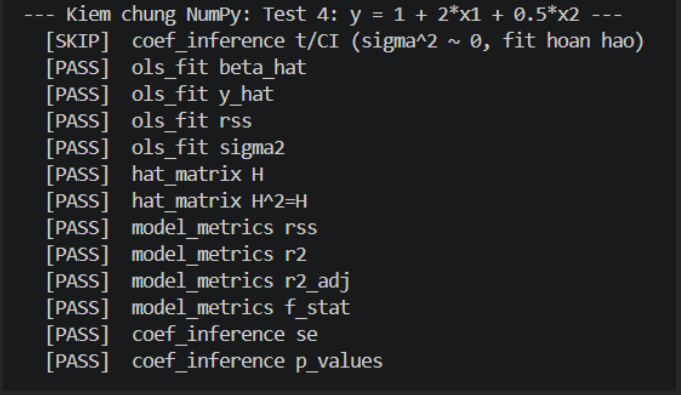
\includegraphics[width=0.75\textwidth]{images/part1/fig_test4_verify.png}
    \caption{Kiểm chứng NumPy -- Test 4.}
    \label{fig:test4_verify}
\end{figure}

\begin{figure}[H]
    \centering
    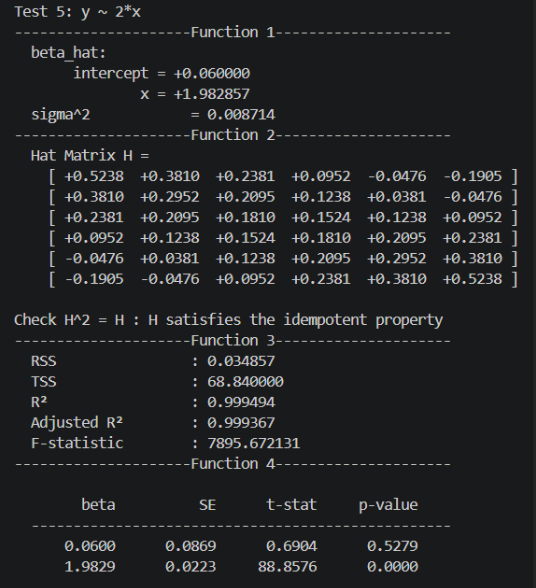
\includegraphics[width=0.85\textwidth]{images/part1/fig_test5_output.png}
    \caption{Kết quả Unit Test 5: $y \approx 2x$ (có nhiễu).
             $\hat{\beta}_0 \approx 0.06$, $\hat{\beta}_1 \approx 1.98$,
             $R^2 \approx 0.9995$.}
    \label{fig:test5_output}
\end{figure}

\begin{figure}[H]
    \centering
    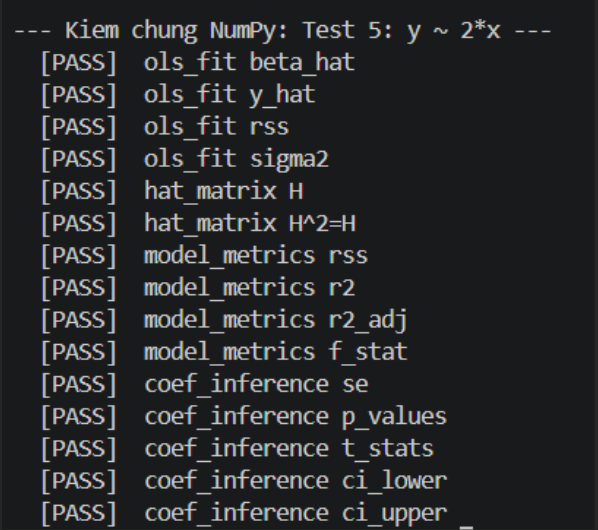
\includegraphics[width=0.75\textwidth]{images/part1/fig_test5_verify.png}
    \caption{Kiểm chứng NumPy -- Test 5: tất cả \texttt{[PASS]}.}
    \label{fig:test5_verify}
\end{figure}
\pagebreak
% ----------------------------------------------------------
\subsection{Hàm \texttt{hat\_matrix(X)}}

\subsubsection{Cơ sở Lý thuyết \& Công thức Toán học}

Hàm \texttt{hat\_matrix} tính ma trận mũ
$\mathbf{H} = \mathbf{X}(\mathbf{X}^\top\mathbf{X})^{-1}\mathbf{X}^\top$
và kiểm tra tính idempotent ($\mathbf{H}^2 = \mathbf{H}$) với ngưỡng sai số
$\mathrm{tol} = 10^{-8}$.
Hàm trả về dictionary: \texttt{H}, \texttt{is\_idempotent}, \texttt{n}, \texttt{k}.

Kết quả kiểm tra trên các unit test đã trình bày ở Yêu cầu 1 đều xác nhận
$\mathbf{H}^2 = \mathbf{H}$ và \texttt{[PASS] hat\_matrix H}, \texttt{[PASS] hat\_matrix H\textasciicircum2=H}.

% ----------------------------------------------------------
\subsection{Hàm \texttt{model\_metrics(y, \^{}y, p)}}

\subsubsection{Cơ sở Lý thuyết \& Công thức Toán học}

Hàm tính các chỉ số đánh giá mô hình: RSS, TSS, $R^2$, $\bar{R}^2$, và
$F$-statistic theo các công thức đã trình bày ở mục~\ref{}.
Hàm trả về dictionary: \texttt{rss}, \texttt{tss}, \texttt{r2}, \texttt{r2\_adj},
\texttt{f\_stat}, \texttt{df\_model}, \texttt{df\_resid}, \texttt{y\_mean}.

Kết quả kiểm chứng trên toàn bộ 5 unit test đều cho \texttt{[PASS]}.

% ----------------------------------------------------------
\subsection{Hàm \texttt{coef\_inference(X, y, \^{}β, σ²)}}

\subsubsection{Cơ sở Lý thuyết \& Công thức Toán học}

Hàm thực hiện kiểm định thống kê cho từng hệ số $\beta_j$:
\begin{enumerate}
    \item Sai số chuẩn: $\mathrm{SE}(\hat{\beta}_j) = \hat{\sigma}\sqrt{[(\mathbf{X}^\top\mathbf{X})^{-1}]_{jj}}$.
    \item $t$-statistic: $t_j = \hat{\beta}_j / \mathrm{SE}(\hat{\beta}_j)$.
    \item $p$-value (hai phía): $p_j = 2\,\mathbb{P}(T > |t_j|)$, $T \sim t_{n-p-1}$.
    \item Khoảng tin cậy 95\%: $\hat{\beta}_j \pm t_{0.025,\,n-p-1} \cdot \mathrm{SE}(\hat{\beta}_j)$.
\end{enumerate}
Hàm dùng phân phối $t$ cài đặt thủ công qua hàm beta không hoàn chỉnh chính quy
(\texttt{\_regularized\_incomplete\_beta}, \texttt{\_t\_cdf}, \texttt{\_t\_sf},
\texttt{\_t\_ppf}).

Kết quả kiểm chứng với SciPy cho \texttt{[PASS]} trên tất cả unit test có
$\hat{\sigma}^2 > 0$ (các test fit hoàn hảo được \texttt{[SKIP]} ở mục $t$/CI).

% ----------------------------------------------------------
\subsection{Hàm \texttt{vif(X)} -- Hệ số Phóng đại Phương sai}

\subsubsection{Cơ sở Lý thuyết \& Công thức Toán học}

Hệ số phóng đại phương sai (Variance Inflation Factor -- VIF) dùng để phát hiện và đo
lường mức độ nghiêm trọng của đa cộng tuyến trong mô hình hồi quy bội.
Công thức tính VIF cho biến $X_i$:
\begin{equation}
    \mathrm{VIF}_i = \frac{1}{1 - R_i^2},
\end{equation}
trong đó $R_i^2$ là hệ số xác định khi thực hiện hồi quy biến $X_i$ theo tất cả các biến
độc lập còn lại trong ma trận đặc trưng $\mathbf{X}$.
Quy tắc: VIF $\geq 5$ (hoặc $10$) là dấu hiệu đa cộng tuyến nghiêm trọng.

\subsubsection{Kết quả Cài đặt \& Kiểm chứng}

\begin{itemize}
    \item \textbf{Triển khai:} Thuật toán được cài đặt thủ công trong module
        \texttt{ols\_implementation.py} thông qua tính toán ma trận nghịch đảo để
        tìm $R_i^2$ cho từng biến.
    \item \textbf{Kiểm chứng:} Khởi tạo dữ liệu giả lập với 3 biến, trong đó
        $X_3$ có tương quan tuyến tính chặt chẽ với $X_1$ và $X_2$.
        Kết quả Unit Test cho thấy hàm tính chính xác VIF rất lớn cho $X_3$.
        Kết quả khớp hoàn toàn (sai số $\approx 0$) so với hàm
        \texttt{variance\_inflation\_factor} của thư viện \texttt{statsmodels}.
\end{itemize}

\begin{figure}[H]
    \centering
    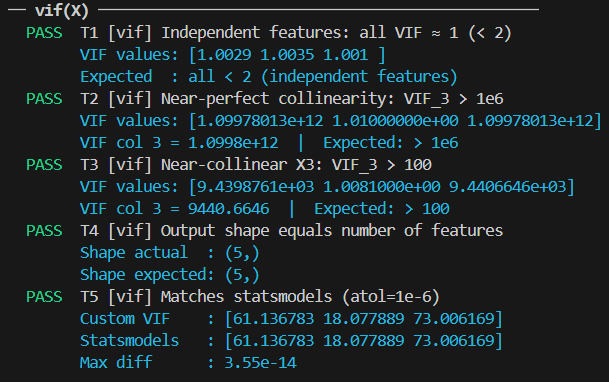
\includegraphics[width=0.85\textwidth]{images/part1/fig_vif_unittest.png}
    \caption{Unit test hàm \texttt{vif}: kết quả kiểm chứng so với \texttt{statsmodels}.}
    \label{fig:vif_unittest}
\end{figure}

% ----------------------------------------------------------
\subsection{Hồi quy Ridge -- Hàm \texttt{ridge\_fit(X, y, lam)}}

\subsubsection{Cơ sở Lý thuyết \& Công thức Toán học}

Khi xảy ra đa cộng tuyến, ma trận $\mathbf{X}^\top\mathbf{X}$ gần suy biến, khiến phương
sai của các ước lượng OLS bị thổi phồng. Hồi quy Ridge khắc phục điều này bằng cách thêm
đại lượng phạt $\lambda \geq 0$ vào đường chéo:
\begin{equation}
    \hat{\boldsymbol{\beta}}_{\mathrm{ridge}}
    = (\mathbf{X}^\top\mathbf{X} + \lambda\mathbf{I})^{-1}\mathbf{X}^\top\mathbf{y}.
\end{equation}
\textbf{Lưu ý:} Trong thực tiễn, intercept không bị phạt; phần tử $(0,0)$ của ma trận
phạt được gán bằng 0.

\subsubsection{Kết quả Cài đặt \& Kiểm chứng}

\begin{itemize}
    \item \textbf{Triển khai:} Hàm \texttt{ridge\_fit} được đóng gói trong module
        \texttt{ridge\_lasso.py}.
    \item \textbf{Kiểm chứng:} Kết quả vector hệ số khớp tuyệt đối với
        \texttt{sklearn.linear\_model.Ridge} (sai số $\approx 10^{-16}$).
    \item \textbf{Ridge Trace:} Đồ thị biểu diễn sự co rút (shrinkage) của các hệ số
        hồi quy khi $\lambda$ tăng dần -- các hệ số tiến về 0, giúp giảm độ phức tạp mô hình.
\end{itemize}

\begin{figure}[H]
    \centering
    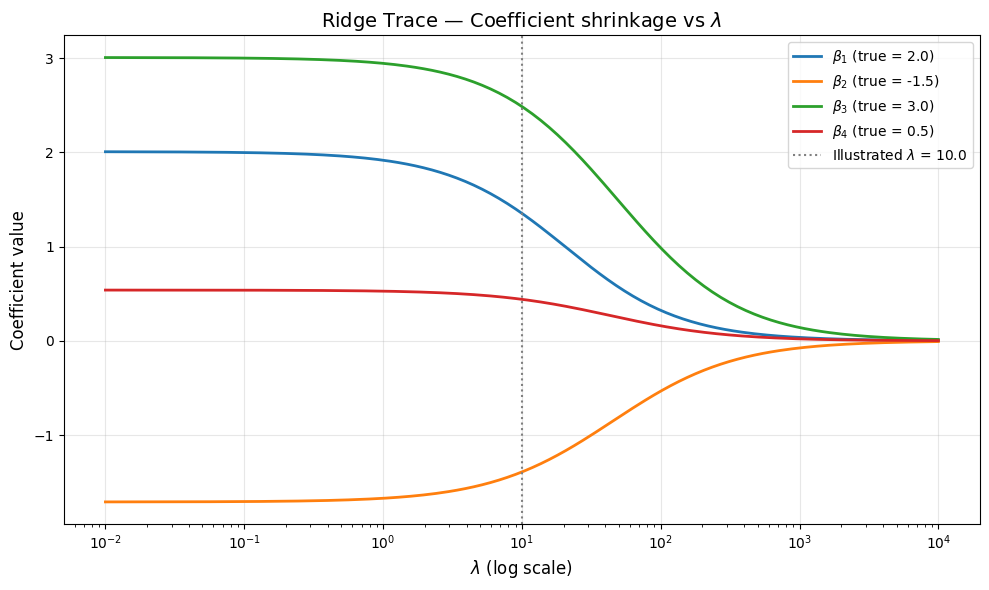
\includegraphics[width=0.85\textwidth]{images/part1/fig_ridge_trace.png}
    \caption{Đồ thị Ridge Trace: sự co rút của các hệ số hồi quy khi tăng mức phạt $\lambda$.}
    \label{fig:ridge_trace}
\end{figure}

\begin{figure}[H]
    \centering
    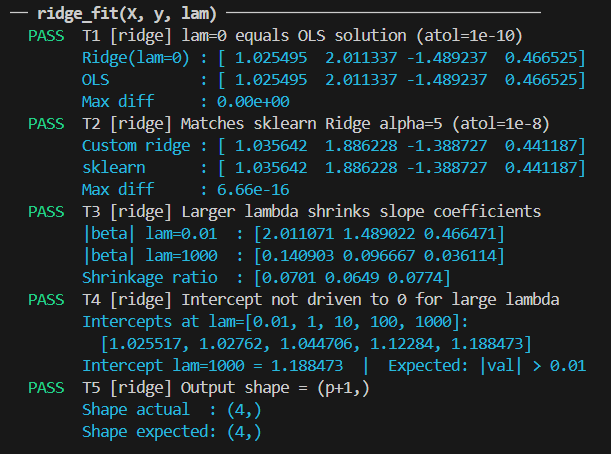
\includegraphics[width=0.85\textwidth]{images/part1/fig_ridge_unittest.png}
    \caption{Unit test hàm \texttt{ridge\_fit}: so sánh với \texttt{sklearn.linear\_model.Ridge}.}
    \label{fig:ridge_unittest}
\end{figure}
\pagebreak

% ----------------------------------------------------------
\subsection{Biểu đồ Phân tích Phần dư -- \texttt{residual\_plots}}

\subsubsection{Cơ sở Lý thuyết \& Công thức Toán học}

Để kiểm tra các giả định của hồi quy tuyến tính, ta sử dụng 4 biểu đồ chẩn đoán chuẩn
mực (theo định dạng \texttt{plot(lm())} trong R):

\begin{enumerate}
    \item \textbf{Residuals vs Fitted:} Kiểm tra tính tuyến tính và đồng phương sai.
        Lý tưởng: phần dư phân tán ngẫu nhiên quanh 0, không có xu hướng.
    \item \textbf{Normal Q-Q:} Kiểm tra phần dư có phân phối chuẩn.
        Lý tưởng: các điểm bám sát đường chéo.
    \item \textbf{Scale-Location:} Kiểm tra homoscedasticity (phương sai đồng đều).
        Lý tưởng: đường xu hướng phẳng.
    \item \textbf{Cook's Distance:} Xác định điểm ngoại lai ảnh hưởng mạnh.
        Công thức:
        \begin{equation}
            D_i = \frac{r_i^2}{p} \cdot \frac{h_{ii}}{1 - h_{ii}},
        \end{equation}
        với $h_{ii}$ là đường chéo của ma trận $\mathbf{H}$,
        $r_i$ là phần dư chuẩn hóa.
        Ngưỡng cảnh báo: $4/n$.
\end{enumerate}

\subsubsection{Kết quả Cài đặt \& Kiểm chứng}

\begin{itemize}
    \item \textbf{Triển khai:} Module \texttt{residual\_analysis.py} tự tính toán phần dư
        chuẩn hóa và ma trận Hat. Đồ thị Cook's Distance dạng bar chart với vạch ngưỡng
        $4/n$ tự động highlight và đánh số các điểm vượt ngưỡng.
    \item \textbf{Kiểm chứng:} Đồ thị Q-Q bám sát đường thẳng (phân phối chuẩn),
        phần dư phân tán ngẫu nhiên, các điểm ngoại lai được đánh dấu tự động.
\end{itemize}

\begin{figure}[H]
    \centering
    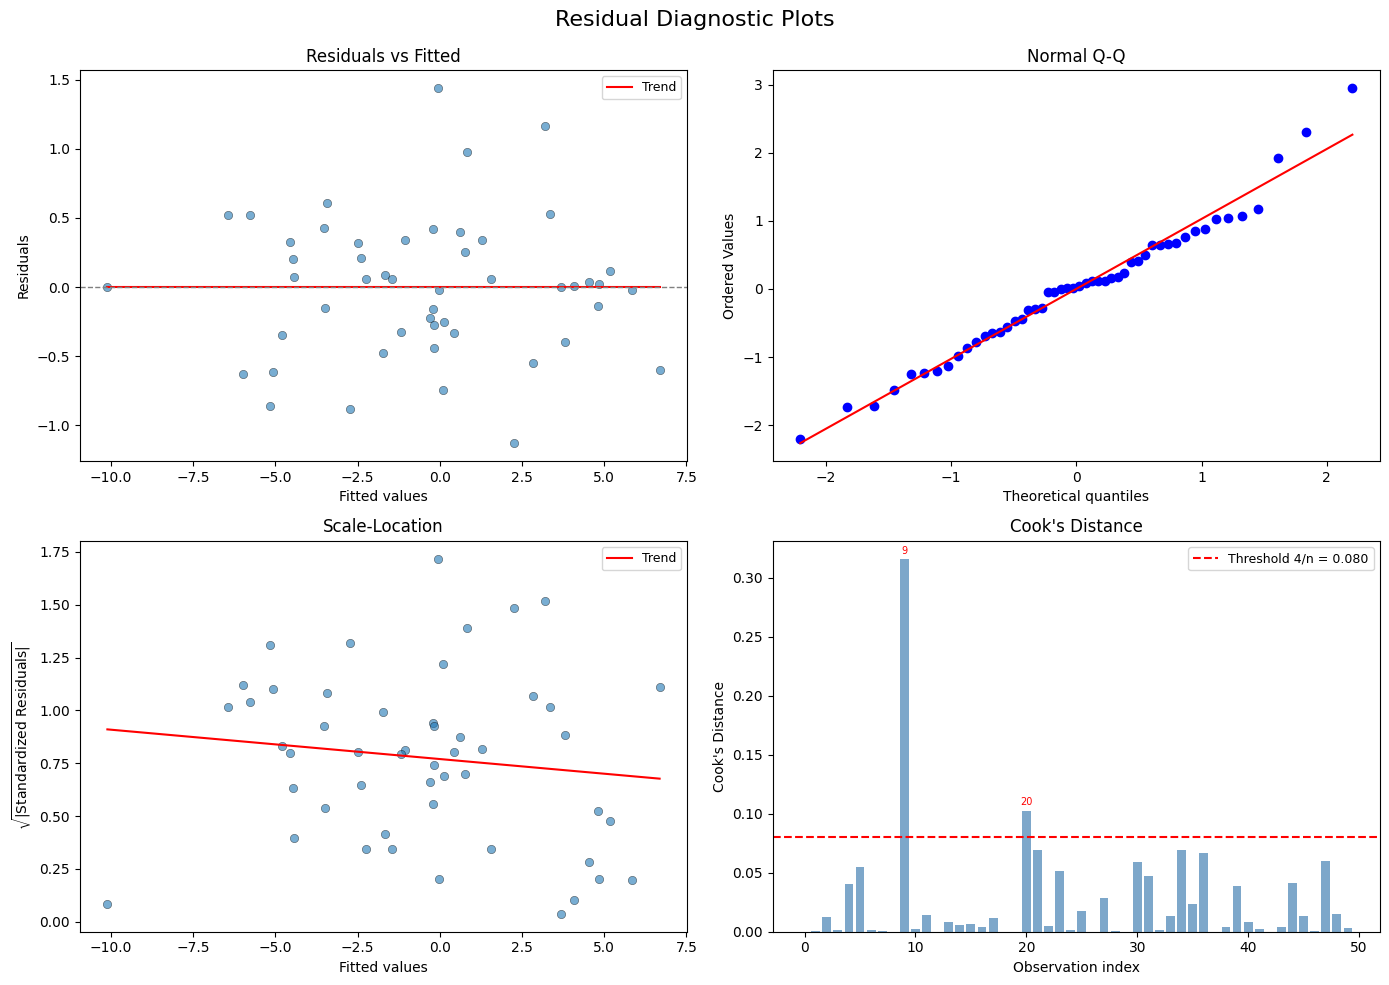
\includegraphics[width=\textwidth]{images/part1/fig_residual_plots.png}
    \caption{Bộ 4 biểu đồ chẩn đoán phần dư của mô hình OLS:
             Residuals vs Fitted, Normal Q-Q, Scale-Location, Cook's Distance.}
    \label{fig:residual_plots}
\end{figure}

\begin{figure}[H]
    \centering
    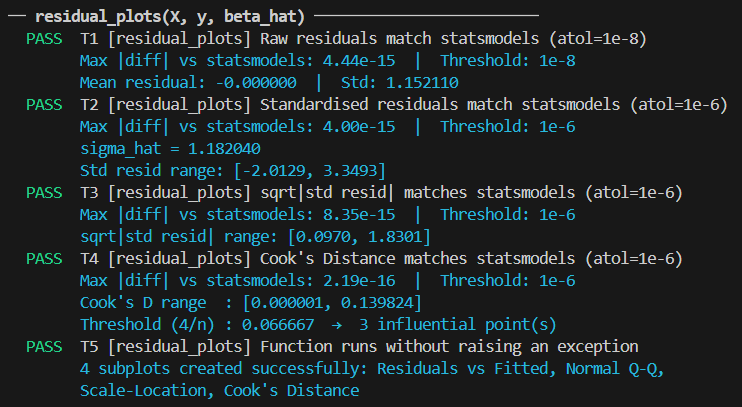
\includegraphics[width=0.85\textwidth]{images/part1/fig_residual_unittest.png}
    \caption{Unit test hàm \texttt{residual\_plots}.}
    \label{fig:residual_unittest}
\end{figure}

% ----------------------------------------------------------
\subsection{Kiểm định chéo K-Fold -- \texttt{kfold\_cv(X, y, k)}}

\subsubsection{Cơ sở Lý thuyết \& Công thức Toán học}

Phương pháp $k$-Fold CV ước lượng khả năng tổng quát hóa của mô hình một cách khách quan
hơn so với chia tập Train/Test đơn lẻ. Tập dữ liệu được chia đều thành $k$ phần ngẫu
nhiên. Vòng lặp $k$ lần lần lượt lấy 1 phần làm tập kiểm tra và $k-1$ phần làm tập huấn luyện.
Điểm đánh giá trung bình:
\begin{equation}
    \mathrm{CV}(k) = \frac{1}{k}\sum_{i=1}^{k}\mathrm{MSE}_i.
\end{equation}

\subsubsection{Kết quả Cài đặt \& Kiểm chứng}

\begin{itemize}
    \item \textbf{Triển khai:} Hàm \texttt{kfold\_cv} trong module
        \texttt{cross\_validation.py}, cố định \texttt{random\_state} qua
        \texttt{numpy.random.default\_rng(random\_state)} đảm bảo tính tái lập
        (reproducibility) hoàn hảo.
    \item \textbf{Kiểm chứng:} MSE trung bình và mảng MSE từng fold hoàn toàn trùng
        khớp với \texttt{cross\_val\_score} của \texttt{sklearn}. Với cùng tham số seed,
        kết quả chia fold giống nhau 100\%.
\end{itemize}

\begin{figure}[H]
    \centering
    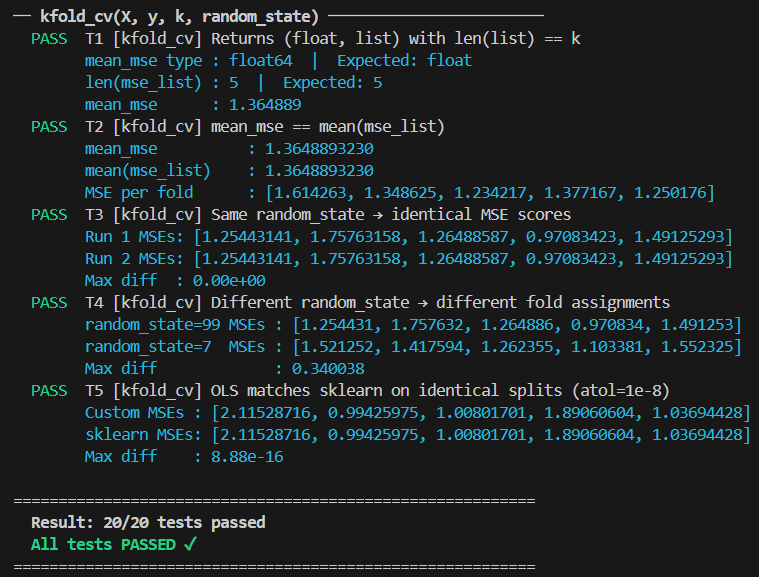
\includegraphics[width=0.85\textwidth]{images/part1/fig_kfold_unittest.png}
    \caption{Unit test hàm \texttt{kfold\_cv}: so sánh với \texttt{sklearn.cross\_val\_score}.}
    \label{fig:kfold_unittest}
\end{figure}

% ----------------------------------------------------------
\subsection{Minh họa Định lý Gauss--Markov (Monte Carlo)}

\subsubsection{Cơ sở Lý thuyết \& Công thức Toán học}

Theo định lý Gauss--Markov, trong số tất cả các ước lượng tuyến tính không chệch của
tham số $\boldsymbol{\beta}$, ước lượng OLS là tốt nhất (BLUE -- Best Linear Unbiased
Estimator) vì có phương sai nhỏ nhất:
\begin{itemize}
    \item \textbf{Không chệch (Unbiased):} $\mathbb{E}[\hat{\boldsymbol{\beta}}] = \boldsymbol{\beta}$.
    \item \textbf{Phương sai nhỏ nhất:}
        $\mathrm{Var}(\hat{\boldsymbol{\beta}}_{\mathrm{OLS}}) \leq \mathrm{Var}(\tilde{\boldsymbol{\beta}})$
        với mọi ước lượng tuyến tính không chệch $\tilde{\boldsymbol{\beta}}$ bất kỳ.
\end{itemize}

\subsubsection{Kết quả Cài đặt Mô phỏng (Monte Carlo)}

\textbf{Quy trình mô phỏng:}
\begin{enumerate}
    \item Thiết lập vòng lặp Monte Carlo $N = 2000$ lần.
    \item Mỗi lần lặp: sinh nhiễu ngẫu nhiên $\boldsymbol{\varepsilon}$, tính
        $\hat{\boldsymbol{\beta}}_{\mathrm{OLS}} = (\mathbf{X}^\top\mathbf{X})^{-1}\mathbf{X}^\top\mathbf{y}$.
    \item Đồng thời xây dựng \textbf{Ước lượng Tuyến tính Trọng số}
        $\hat{\boldsymbol{\beta}}_W = (\mathbf{W}^\top\mathbf{X})^{-1}\mathbf{W}^\top\mathbf{y}$
        với $\mathbf{W}$ là ma trận nhiễu. Cả hai đều tuyến tính và không chệch.
\end{enumerate}

\textbf{Kết luận mô phỏng:}
\begin{itemize}
    \item \textbf{Kiểm chứng không chệch:} Trung bình 2000 lần lặp của cả
        $\hat{\boldsymbol{\beta}}_{\mathrm{OLS}}$ và $\hat{\boldsymbol{\beta}}_W$ đều hội
        tụ rất sát về vector $\boldsymbol{\beta}$ thực tế.
    \item \textbf{Kiểm chứng phương sai (BLUE):} Phương sai của OLS luôn thấp hơn
        ước lượng trọng số. Trên đồ thị mật độ KDE, phân phối của OLS hẹp hơn,
        cao hơn, chứng tỏ OLS ít biến thiên và đáng tin cậy hơn.
\end{itemize}

\begin{figure}[H]
    \centering
    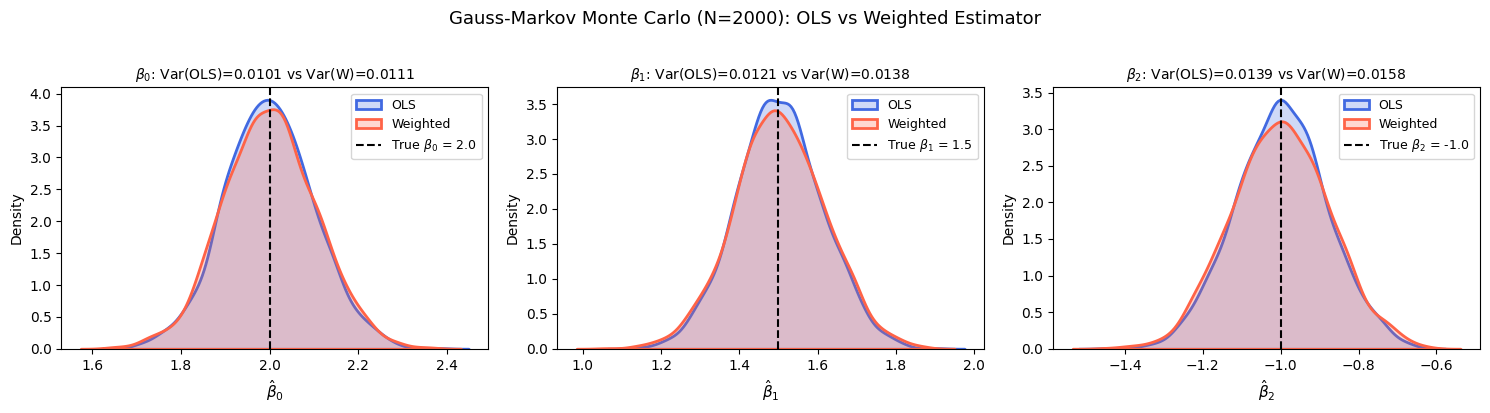
\includegraphics[width=\textwidth]{images/part1/fig_gauss_markov_kde.png}
    \caption{Biểu đồ mật độ phân phối (KDE) so sánh phương sai của OLS và ước lượng trọng số
             qua 2000 lần mô phỏng Monte Carlo.
             Phân phối OLS (đường hẹp, cao) cho thấy phương sai nhỏ hơn rõ rệt.}
    \label{fig:gauss_markov_kde}
\end{figure}

\begin{figure}[H]
    \centering
    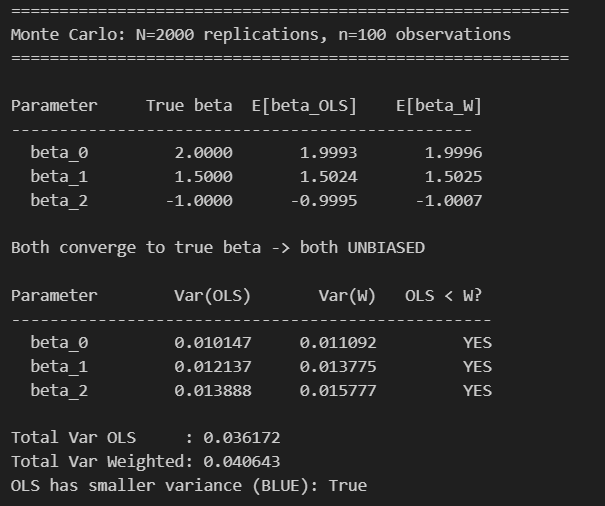
\includegraphics[width=0.85\textwidth]{images/part1/fig_gauss_markov_result.png}
    \caption{Kết quả chạy minh họa định lý Gauss--Markov bằng Monte Carlo:
             giá trị trung bình $\hat{\boldsymbol{\beta}}$ và so sánh phương sai.}
    \label{fig:gauss_markov_result}
\end{figure}
\pagebreak
\section{Phần 2: Ứng Dụng Data Fitting vào Dữ Liệu Thực Tế}
\subsection*{Đề tài: Phân tích và Dự đoán Lương Developer (Stack Overflow Survey 2023)}

% ----------------------------------------------------------
\subsection{Giới Thiệu Bài Toán}

\subsubsection{Lý do chọn dataset}

\textbf{Stack Overflow Developer Survey 2023} được chọn vì đáp ứng đầy đủ
các tiêu chí của đề bài:

\begin{table}[H]
\centering
\begin{tabular}{lp{9cm}}
\toprule
\textbf{Tiêu chí} & \textbf{Đáp ứng} \\
\midrule
Dữ liệu thực (real-world) & Khảo sát 89.184 lập trình viên toàn cầu, thu thập năm 2023 \\
Có missing values $\geq 5\%$ & \texttt{ConvertedCompYearly} thiếu 46\%, \texttt{ICorPM} thiếu 51\% \\
Biến mục tiêu liên tục & \texttt{ConvertedCompYearly} — lương năm (USD) \\
$n \geq 200$, $p \geq 3$ & $n = 89.184$ quan sát, $p = 9$ features dự báo \\
Nguồn đáng tin cậy & Công bố chính thức tại \texttt{survey.stackoverflow.co/2023} \\
\bottomrule
\end{tabular}
\caption{Kiểm tra tiêu chí chọn dataset.}
\end{table}

\noindent\textbf{Lý do thực tế:} Bài toán dự đoán lương developer có ý nghĩa ứng dụng
cao — phản ánh câu hỏi thực tế ``yếu tố nào ảnh hưởng nhiều nhất đến thu nhập trong
ngành IT?''

\subsubsection{Mô tả features}

\begin{table}[H]
\centering
\begin{tabular}{llp{8.5cm}}
\toprule
\textbf{Cột} & \textbf{Kiểu} & \textbf{Mô tả} \\
\midrule
\texttt{ConvertedCompYearly} & Numeric & \textbf{Biến mục tiêu} — lương năm quy đổi sang USD \\
\texttt{YearsCodePro} & String$\to$Numeric & Số năm kinh nghiệm lập trình chuyên nghiệp \\
\texttt{WorkExp} & Numeric & Tổng số năm đi làm \\
\texttt{EdLevel} & Ordinal & Trình độ học vấn — 7 nhãn survey, encode về 6 bậc ordinal (1–6) \\
\texttt{DevType} & Multi-select & Loại lập trình viên \\
\texttt{OrgSize} & Ordinal & Quy mô tổ chức (số nhân viên) \\
\texttt{Country} & Nominal & Quốc gia làm việc \\
\texttt{RemoteWork} & Nominal & Hình thức làm việc (remote/hybrid/onsite) \\
\texttt{ICorPM} & Binary & Individual Contributor hay People Manager \\
\texttt{Employment} & Multi-select & Hình thức hợp đồng \\
\bottomrule
\end{tabular}
\caption{Mô tả các features trong bộ dữ liệu.}
\end{table}

% ----------------------------------------------------------
\subsection{Phân Tích Dữ Liệu (EDA)}

\subsubsection{Thống kê mô tả}

\begin{table}[H]
\centering
\begin{tabular}{lr}
\toprule
\textbf{Chỉ số} & \textbf{Giá trị} \\
\midrule
Số quan sát & 89.184 \\
Median lương & \$74.963 \\
Mean lương & \$103.110 \\
Max lương & \$74.351.427 \\
Std lương & \$681.419 \\
\bottomrule
\end{tabular}
\caption{Thống kê mô tả biến mục tiêu \texttt{ConvertedCompYearly}.}
\end{table}

Khoảng cách lớn giữa mean và median, cùng giá trị max cực đoan (\$74M so với median
\$75K — tỉ lệ \textbf{1000:1}), cho thấy phân phối \textbf{lệch phải rất mạnh} — đặc
trưng điển hình của dữ liệu thu nhập.

\subsubsection{Phân tích missing values}

\begin{figure}[H]
    \centering
    
\includegraphics[width=\textwidth]{images/part2/fig1_missing_rate.png}
    \caption{Tỉ lệ missing value theo từng cột. Thanh đỏ = vượt ngưỡng 5\%.
             7/10 cột có tỉ lệ thiếu đáng kể; đặc biệt \texttt{ConvertedCompYearly}
             (biến mục tiêu) thiếu 46\% và \texttt{RemoteWork} thiếu 17.2\%.}
    \label{fig:missing_rate}
\end{figure}

\begin{table}[H]
\centering
\begin{tabular}{lrl}
\toprule
\textbf{Cột} & \textbf{Tỉ lệ thiếu} & \textbf{Cơ chế} \\
\midrule
\texttt{ConvertedCompYearly} & 46.2\% & MNAR \\
\texttt{ICorPM} & 51.0\% & MAR \\
\texttt{WorkExp} & 51.1\% & MAR \\
\texttt{YearsCodePro} & 25.9\% & MAR \\
\texttt{OrgSize} & 27.0\% & MAR \\
\texttt{DevType} & 13.8\% & MAR \\
\texttt{RemoteWork} & 17.2\% & MAR \\
\texttt{Country}, \texttt{EdLevel}, \texttt{Employment} & $< 2\%$ & MCAR \\
\bottomrule
\end{tabular}
\caption{Tỉ lệ và cơ chế missing của từng cột.}
\end{table}

\subsubsection{Phân tích cơ chế missing và lý do xử lý}

\paragraph{MCAR (Missing Completely At Random).}
\texttt{Country}, \texttt{RemoteWork}, \texttt{EdLevel} có tỉ lệ thiếu $< 2\%$,
không có pattern hệ thống.
$\to$ \textbf{Quyết định:} Listwise deletion — mất không đáng kể, không gây bias.

\paragraph{MAR (Missing At Random).}
MAR (Missing At Random). \texttt{WorkExp}, \texttt{YearsCodePro}, \texttt{ICorPM}, \texttt{OrgSize}, \texttt{RemoteWork} thiếu nhiều hơn ở nhóm freelancer và sinh viên — missingness tương quan với biến \texttt{Employment} (có thể quan sát được). \texttt{WorkExp} và \texttt{YearsCodePro} thiếu ở những người không có kinh nghiệm lập trình chuyên nghiệp; \texttt{RemoteWork} thiếu 17.2\% ở nhóm không phải full-time employee.
$\to$ \textbf{Quyết định:} Drop hàng sau khi encode vì nhóm này thường không phải
full-time developer, và tỉ lệ mất thêm chỉ $< 5\%$.

\paragraph{MNAR (Missing Not At Random).}
\texttt{ConvertedCompYearly} — xác suất không khai báo phụ thuộc vào chính giá trị
lương: người lương rất cao hoặc rất thấp có xu hướng bỏ qua.
$\to$ \textbf{Quyết định:} Bắt buộc dùng listwise deletion — \textbf{không thể impute
biến mục tiêu} vì bất kỳ imputation nào cũng làm méo phân phối $y$ và khiến các
metric trên test set không còn tin cậy.

\subsubsection{Phát hiện outlier}

\begin{figure}[H]
    \centering
    
\includegraphics[width=\textwidth]{images/part2/fig3_outlier_detection.png}
    \caption{So sánh phương pháp phát hiện outlier: IQR (ngưỡng \$238.242, phát hiện
             4.6\% mẫu) vs.\ Z-score (ngưỡng $3\sigma \approx \$2.1\text{M}$,
             chỉ phát hiện 0.1\%).}
    \label{fig:outlier}
\end{figure}

\noindent\textbf{IQR (Interquartile Range):}
\[
    Q_1 = \$43.907, \quad Q_3 = \$121.641, \quad \mathrm{IQR} = \$77.734
\]
\[
    \text{Upper bound} = Q_3 + 1.5 \times \mathrm{IQR} = \$238.242
    \quad \Rightarrow \quad \text{Outliers: } 4.6\%\ (2.208 \text{ quan sát})
\]

\noindent\textbf{Z-score:} Ngưỡng $3\sigma \approx \$2.144.657$ — quá bảo thủ vì \texttt{std}
bị thổi phồng bởi giá trị \$74M, chỉ phát hiện 0.1\% outlier.

\noindent\textbf{Lý do chọn IQR:} IQR chỉ dùng $Q_1$ và $Q_3$, không bị ảnh hưởng bởi
outlier cực đoan. Z-score không phù hợp cho phân phối lệch phải mạnh vì giá trị max
thổi phồng \texttt{std}, khiến ngưỡng $3\sigma \approx \$2.1\text{M}$ — cho phép hầu
hết giá trị cực đoan đi qua.

\subsubsection{Phân tích tương quan}

\begin{figure}[H]
    \centering
    
\includegraphics[width=0.6\textwidth]{images/part2/fig4_correlation_heatmap.png}
    \caption{Ma trận tương quan Pearson giữa các biến số. Cặp
             \texttt{YearsCodePro}--\texttt{WorkExp} có $r \approx 0.928$ — tương
             quan cao nhưng không cần loại bỏ ngay ở bước này.}
    \label{fig:heatmap}
\end{figure}

\begin{table}[H]
\centering
\begin{tabular}{llp{7cm}}
\toprule
\textbf{Cặp biến} & $r$ & \textbf{Nhận xét} \\
\midrule
\texttt{YearsCodePro} $\leftrightarrow$ \texttt{WorkExp} & $\approx 0.928$ & Tương quan cao; cần kiểm tra VIF sau encoding \\
\texttt{ConvertedCompYearly} $\leftrightarrow$ \texttt{YearsCodePro} & $\approx 0.039$ & Tương quan rất yếu — salary phụ thuộc chủ yếu vào Country và role, không phải kinh nghiệm đơn thuần \\
\texttt{ConvertedCompYearly} $\leftrightarrow$ \texttt{WorkExp} & $\approx 0.046$ & Tương quan rất yếu — tương tự YearsCodePro \\
\bottomrule
\end{tabular}
\caption{Nhận xét về các cặp tương quan đáng chú ý.}
\end{table}

\noindent Không có cặp nào có $|r| > 0.9$ ngoài cặp YearsCodePro--WorkExp — không cần loại
bỏ feature nào ở bước này. Sau khi one-hot encode, VIF được kiểm tra lại.

% ----------------------------------------------------------
\subsection{Tiền Xử Lý Dữ Liệu}

\subsubsection{Pipeline tổng thể}

\begin{figure}[H]
    \centering
    
\includegraphics[width=\textwidth]{images/part2/fig5_pipeline_diagram.png}
    \caption{Sơ đồ DataPipeline toàn bộ quá trình tiền xử lý: từ 89.184 hàng raw
             data đến 38.415 train / 9.604 test với 38 features.}
    \label{fig:pipeline}
\end{figure}

Quy trình xử lý theo thứ tự:

\begin{enumerate}
    \item Listwise deletion (\texttt{ConvertedCompYearly = NaN}) $\to$ 48.019 hàng
    \item Winsorize tại \$238.242
    \item \texttt{log1p} transform $\to$ biến mục tiêu $y$
    \item Encode features (ordinal / binary / one-hot)
    \item Drop NaN hàng còn lại (MAR)
    \item 80/20 train/test split (\texttt{random\_state=42})
    \item StandardScaler (fit on train, transform test)
    \item[$\Rightarrow$] Dataset sạch: \textbf{38.415 train | 9.604 test | 38 features}
\end{enumerate}

\subsubsection{Winsorization và Log1p Transform}

\begin{figure}[H]
    \centering
    
\includegraphics[width=\textwidth]{images/part2/fig2_salary_transform.png}
    \caption{Pipeline biến đổi phân phối lương: (trái) raw salary lệch phải mạnh;
             (giữa) sau Winsorization tại cap = \$238.242;
             (phải) sau \texttt{log1p} transform — phân phối gần chuẩn hơn.}
    \label{fig:salary_transform}
\end{figure}

\noindent\textbf{Lý do chọn Winsorization thay vì xóa hàng:}
\begin{itemize}
    \item Xóa 4.6\% hàng làm mất thêm dữ liệu (vốn đã giảm mạnh do MNAR)
    \item Winsorization giữ toàn bộ hàng, chỉ co giá trị extreme về ngưỡng hợp lý
    \item Giá trị \$74M rất có thể là lỗi nhập liệu (tỉ lệ 1000:1 so với median)
\end{itemize}

\noindent\textbf{Lý do dùng \texttt{log1p}:}
\begin{itemize}
    \item Nén đuôi phải $\to$ phân phối target $y$ gần normal hơn
        (mean $\approx 11$, std $\approx 0.8$ sau transform)
    \item Residuals đáp ứng giả thuyết Gauss--Markov tốt hơn
    \item Hệ số có ý nghĩa nhân: tăng 1 đơn vị feature $\to$ lương nhân với
        $e^{\hat{\beta}_j}$
    \item Dùng \texttt{log1p} thay \texttt{log} để xử lý an toàn trường hợp salary = 0
\end{itemize}

\subsubsection{Feature Encoding}

\begin{table}[H]
\centering
\begin{tabular}{llp{7.5cm}}
\toprule
\textbf{Feature} & \textbf{Phương pháp} & \textbf{Lý do} \\
\midrule
\texttt{EdLevel} & Ordinal (1--6) & Có thứ tự tự nhiên: tiểu học $<$ THPT $<$ ĐH $<$ ThS $<$ TS; tiết kiệm 5 dummy columns (so với one-hot 6 bậc) \\
\texttt{OrgSize} & Ordinal (1--9) & Thứ tự quy mô nhân viên rõ ràng \\
\texttt{ICorPM} & Binary (0/1) & Chỉ có 2 giá trị \\
\texttt{Employment} & Binary \texttt{is\_fulltime} & 106 unique values; chỉ quan tâm full-time vs không \\
\texttt{DevType} & One-hot top-10 + Other & Multi-select; top-10 chiếm $> 90\%$ \\
\texttt{Country} & One-hot top-20 + Other & 185 quốc gia; top-20 chiếm $\approx 83\%$ data \\
\texttt{RemoteWork} & One-hot (3 loại) & Nominal, không có thứ tự tự nhiên \\
\bottomrule
\end{tabular}
\caption{Chiến lược encoding cho từng feature.}
\end{table}

\subsubsection{Class DataPipeline — Tránh Data Leakage}

Class \texttt{DataPipeline} tách biệt \texttt{fit} và \texttt{transform}:

\begin{itemize}
    \item \texttt{fit(X\_train)}: Học top-10 DevType, top-20 Country và fit
        \texttt{StandardScaler} \textbf{chỉ từ tập train}.
    \item \texttt{transform(X)}: Áp dụng encoding đã học — không học lại.
        Các category chưa thấy được gán 0.
\end{itemize}

\noindent\textbf{Tại sao phải tách fit/transform:} Nếu học top categories từ toàn bộ
dataset (kể cả test set), model sẽ ``biết trước'' phân phối của test — đây là
\textbf{data leakage}, khiến metric trên test lạc quan giả tạo.

\noindent\textbf{Lý do chọn 80/20 split với \texttt{random\_state=42}:} Train set đủ lớn để
học pattern, test set đủ để đánh giá tin cậy; random seed cố định đảm bảo
reproducibility.

\noindent\textbf{Lý do dùng StandardScaler (z-score) thay vì MinMaxScaler:} Ridge và Lasso
có penalty trên norm hệ số — nếu không scale, feature có đơn vị lớn bị shrink nhiều hơn
feature nhỏ, gây bias. StandardScaler cũng ổn định hơn khi có outlier.

% ----------------------------------------------------------
\subsection{Xây Dựng Mô Hình}

\subsubsection{M1 — OLS Full (Baseline)}

OLS tối thiểu hóa tổng bình phương phần dư:
\begin{equation}
    \hat{\boldsymbol{\beta}} = (\mathbf{X}^\top\mathbf{X})^{-1}\mathbf{X}^\top\mathbf{y}.
\end{equation}

\noindent\textbf{Lý do làm baseline:} OLS không có tham số cần tune, không regularization —
đây là điểm xuất phát để đánh giá xem regularization có cải thiện không.

\noindent\textbf{Kết quả:} $R^2 = 0.3847$, MAE $= 0.538$, RMSE $= 0.945$.

\subsubsection{M2 — OLS Selected (p-value + VIF)}

Lọc feature theo 2 bước:

\textbf{Bước 1 — P-value $< 0.05$:} Loại bỏ feature không có ý nghĩa thống kê.
Với $n \approx 38\text{K}$, test rất nhạy — ngưỡng 0.05 vẫn có thể giữ lại nhiều features.

\textbf{Bước 2 — VIF $\leq 10$:}
\begin{equation}
    \mathrm{VIF}_j = \frac{1}{1 - R_j^2}.
\end{equation}
VIF $> 10$ nghĩa là feature $j$ có thể được giải thích $> 90\%$ bởi các features khác
$\to$ hệ số không ổn định. Ngưỡng 10 được chấp nhận rộng rãi trong tài liệu
(Hair et al., 2009).

\noindent\textbf{Kết quả:} Giữ $\approx 30/38$ features.
$R^2 = 0.3842$, MAE $= 0.539$, RMSE $= 0.946$.

\subsubsection{M3 — Ridge (L2) và Lasso (L1)}

\textbf{Hàm mục tiêu Ridge:}
\begin{equation}
    \min_{\boldsymbol{\beta}} \|\mathbf{y} - \mathbf{X}\boldsymbol{\beta}\|^2
    + \alpha\|\boldsymbol{\beta}\|_2^2.
\end{equation}

\textbf{Hàm mục tiêu Lasso:}
\begin{equation}
    \min_{\boldsymbol{\beta}} \|\mathbf{y} - \mathbf{X}\boldsymbol{\beta}\|^2
    + \alpha\|\boldsymbol{\beta}\|_1.
\end{equation}

\noindent\textbf{Lý do dùng regularization sau OLS:} Sau one-hot encoding có nhiều
correlated dummy columns (các Country gần nhau về lương) $\to$ OLS dễ overfitting.
Ridge co đều tất cả hệ số; Lasso đưa một số về đúng 0 (tự động feature selection).

\textbf{Lý do chọn $\alpha$ bằng 5-fold CV:}

\begin{figure}[H]
    \centering
    
\includegraphics[width=0.75\textwidth]{images/part2/fig9_ridge_alpha_cv.png}
    \caption{Ridge CV — Alpha Selection. Best $\alpha = 0.6136$ tại điểm MSE thấp
             nhất trên thang log. CV MSE tăng mạnh khi $\alpha > 10$.}
    \label{fig:ridge_cv}
\end{figure}

$\alpha$ quá nhỏ $\to$ gần như OLS (underfitting); $\alpha$ quá lớn $\to$ co tất cả về 0.
CV tìm điểm cân bằng bias--variance tối ưu.

\noindent\textbf{Kết quả Ridge:} $\alpha = 0.6136$,
$R^2 = 0.3847$, MAE $= 0.538$, RMSE $= 0.945$.

\noindent\textbf{Kết quả Lasso:} $\alpha = 0.001$, zeroed 6/38 features,
$R^2 = 0.3827$, MAE $= 0.541$, RMSE $= 0.947$.

\subsubsection{M4 — Polynomial Features + Ridge (Bonus)}

Tạo interaction terms và bậc hai:
\[
    \{x_1, \ldots, x_p\} \;\longrightarrow\;
    \{x_1,\, x_1^2,\, x_1 x_2,\, \ldots\}
\]

\noindent\textbf{Lý do thêm polynomial features:} Correlation heatmap cho thấy
\texttt{YearsCodePro} và \texttt{WorkExp} chỉ có $r \approx 0.25$ với salary — quan hệ
có thể phi tuyến hoặc phụ thuộc biến khác (ví dụ: kinh nghiệm $\times$ quốc gia).
Degree $= 2$ (không phải 3+) để tránh bùng nổ features và overfitting.

\noindent\textbf{Lý do kết hợp với Ridge:} $38 \to 779$ features sau expansion
$\to$ Ridge bắt buộc để tránh overfitting.

\noindent\textbf{Kết quả:} $R^2 = 0.4309$, MAE $= 0.500$, RMSE $= 0.909$
\textbf{(tốt nhất)}.

\subsubsection{M5b — Bayesian Ridge (Bonus)}

Đặt prior cho $\boldsymbol{\beta}$:
\begin{equation}
    \boldsymbol{\beta} \sim \mathcal{N}(\mathbf{0}, \lambda^{-1}\mathbf{I}),
    \qquad
    y \mid \mathbf{x}, \boldsymbol{\beta} \sim \mathcal{N}(\mathbf{x}^\top\boldsymbol{\beta},\, \sigma^2).
\end{equation}

\noindent\textbf{Lý do dùng Bayesian Ridge:} Không chỉ cho điểm dự đoán mà còn cung cấp
\textbf{độ không chắc chắn} (predictive std) — ứng dụng thực tế: hệ thống HR biết
``model tin tưởng bao nhiêu'' vào dự đoán này.

\noindent\textbf{Kết quả:} $R^2 = 0.3846$, MAE $= 0.538$, RMSE $= 0.945$.

% ----------------------------------------------------------
\subsection{Đánh Giá và So Sánh Mô Hình}

\subsubsection{Bảng tổng hợp}

\begin{figure}[H]
    \centering
    
\includegraphics[width=\textwidth]{images/part2/fig6_model_comparison.png}
    \caption{So sánh hiệu năng các mô hình trên tập test: $R^2$ (trái),
             MAE và RMSE (phải). Polynomial+Ridge vượt trội rõ rệt.}
    \label{fig:model_comparison}
\end{figure}

\begin{table}[H]
\centering
\begin{tabular}{clccc}
\toprule
\textbf{Hạng} & \textbf{Mô hình} & \textbf{MAE} & \textbf{RMSE} & $R^2$ \\
\midrule
1 & M4 Polynomial+Ridge & 0.5003 & 0.9090 & \textbf{0.4309} \\
2 & M1 OLS Full & 0.5378 & 0.9452 & 0.3847 \\
3 & M3 Ridge & 0.5378 & 0.9452 & 0.3847 \\
4 & M5b Bayesian Ridge & 0.5379 & 0.9452 & 0.3846 \\
5 & M2 OLS Selected & 0.5389 & 0.9456 & 0.3842 \\
6 & M3 Lasso & 0.5407 & 0.9467 & 0.3827 \\
\bottomrule
\end{tabular}
\caption{Tổng hợp hiệu năng các mô hình trên tập test (thang log salary).
         RMSE $\approx 0.91$ trên thang log-salary tương ứng sai số nhân khoảng $\times 2.5$ trên thang gốc (tại vùng median $\sim\$73\text{K}$: khoảng dự đoán từ $\sim\$29\text{K}$ đến $\sim\$181\text{K}$).}
\end{table}

\noindent\textbf{Nhận xét:}
\begin{itemize}
    \item M4 Polynomial+Ridge vượt trội rõ ($R^2 = 0.43$ vs $0.38$ của các mô hình
        tuyến tính) — xác nhận có interaction effects phi tuyến.
    \item OLS Full và Ridge cho kết quả gần như nhau $\to$ multicollinearity không
        nghiêm trọng sau khi đã lọc VIF.
    \item Lasso kém nhất vì $\alpha = 0.001$ — gần như OLS, nhưng mất ổn định của Ridge.
\end{itemize}

\subsubsection{Phân tích phần dư (Ridge — mô hình tuyến tính tốt nhất)}

\begin{figure}[H]
    \centering
    
\includegraphics[width=\textwidth]{images/part2/fig7_residual_plots.png}
    \caption{Bộ 4 biểu đồ chẩn đoán phần dư của mô hình Ridge (mô hình tuyến tính
             tốt nhất): Residuals vs Fitted, Normal Q-Q, Scale-Location,
             Residual Distribution.}
    \label{fig:residual_plots}
\end{figure}

\begin{table}[H]
\centering
\begin{tabular}{lp{5cm}p{6.5cm}}
\toprule
\textbf{Biểu đồ} & \textbf{Quan sát} & \textbf{Nhận xét} \\
\midrule
Residuals vs Fitted & Phân tán quanh 0, có hơi funnel nhỏ ở hai đầu & Quan hệ tuyến tính ổn; heteroscedasticity nhẹ do một số segment lương khó dự đoán \\
Normal Q-Q Plot & Đuôi nặng ở cả hai đầu (heavy tails) & Không hoàn toàn normal; phổ biến với dữ liệu thu nhập. Với $n \approx 38\text{K}$, CLT đảm bảo inference vẫn hợp lệ \\
Scale-Location & Đường xu hướng gần phẳng & Homoscedasticity chấp nhận được sau log-transform \\
Histogram & Gần bell-shape, hơi lệch trái & Mô hình under-predict một số mức lương cao tuyệt đối \\
\bottomrule
\end{tabular}
\caption{Nhận xét bộ 4 biểu đồ phân tích phần dư.}
\end{table}

\noindent\textbf{Lưu ý về Shapiro-Wilk:} Với $n \approx 38\text{K}$, test luôn reject
$H_0$ — không có ý nghĩa thực tế. Quan sát Q-Q plot đáng tin cậy hơn.

\subsubsection{Feature Importance}

\begin{figure}[H]
    \centering
    
\includegraphics[width=\textwidth]{images/part2/fig8_feature_importance.png}
    \caption{Top 20 features quan trọng nhất của mô hình Ridge (theo
             $|\text{coefficient}|$ sau chuẩn hóa). Đỏ = Country, Xanh dương = Numeric,
             Xanh lá = Other.}
    \label{fig:feature_importance}
\end{figure}

\noindent\textbf{Top insights:}
\begin{enumerate}
    \item \textbf{Country} — yếu tố lớn nhất, vượt trội so với kinh nghiệm
        (India, Brazil, Italy dẫn đầu về độ lớn hệ số âm/dương).
    \item \textbf{YearsCodePro} — kinh nghiệm lập trình có ảnh hưởng đáng kể
        (feature numeric quan trọng nhất).
    \item \textbf{RemoteWork\_In-person} — hệ số âm: làm onsite thường thấp hơn
        hybrid/remote (geographic arbitrage).
    \item \textbf{ICorPM} — People Manager có lương cao hơn Individual Contributor.
\end{enumerate}

\noindent\textbf{Kết luận quan trọng:} \textit{``Bạn làm việc ở đâu quan trọng hơn
bạn giỏi đến đâu''} — Country coefficients lớn hơn YearsCodePro đáng kể.

% ----------------------------------------------------------
\subsection{Unit Tests}

30 unit tests được viết cho 6 hàm/class, so sánh kết quả với thư viện chuẩn:

\begin{table}[H]
\centering
\begin{tabular}{clll}
\toprule
\textbf{\#} & \textbf{Hàm} & \textbf{Thư viện đối chiếu} & \textbf{Số test} \\
\midrule
1 & \texttt{winsorize\_series} & \texttt{numpy.clip} & 5 \\
2 & \texttt{log1p\_transform} & \texttt{numpy.log1p} & 5 \\
3 & \texttt{ordinal\_encode} & \texttt{pandas.Series.map} & 5 \\
4 & \texttt{compute\_metrics} & \texttt{sklearn.metrics} & 5 \\
5 & \texttt{compute\_vif} & \texttt{statsmodels.variance\_inflation\_factor} & 5 \\
6 & \texttt{DataPipeline} & sklearn API contract & 5 \\
\midrule
 & \textbf{Tổng} & & \textbf{30/30 PASSED} \\
\bottomrule
\end{tabular}
\caption{Tổng hợp kết quả unit tests Phần 2.}
\end{table}

% ----------------------------------------------------------
\subsection{Kết Luận}

\subsubsection{Tóm tắt kết quả}

\begin{itemize}
    \item Mô hình tốt nhất: \textbf{Polynomial+Ridge} với $R^2 = 0.43$,
        RMSE $= 0.909$ trên log-salary scale.
    \item Mô hình tuyến tính tốt nhất: \textbf{Ridge/OLS Full} với $R^2 = 0.385$ —
        regularization cải thiện nhưng không đột phá so với OLS trên dataset này.
\end{itemize}

\subsubsection{Bài học rút ra}

\begin{enumerate}
    \item \textbf{Preprocessing quan trọng hơn model choice} — Winsorize, log1p và
        \texttt{DataPipeline} class ảnh hưởng đến kết quả nhiều hơn việc chọn Ridge hay Lasso.
    \item \textbf{Geographic arbitrage là thực} — Country coefficient lớn nhất;
        developer ở USA/Switzerland kiếm được nhiều hơn đáng kể so với cùng trình độ
        ở nước khác.
    \item \textbf{Polynomial features bắt được interaction effects thực sự} —
        $R^2$ tăng 0.046 điểm; kinh nghiệm $\times$ quốc gia và các tương tác khác
        có ý nghĩa thực tế.
    \item \textbf{DataPipeline class là thiết kế đúng cho production} — tách
        fit/transform ngăn data leakage, đảm bảo pipeline có thể tái dùng với dữ liệu mới.
\end{enumerate}

\subsubsection{Hướng mở rộng}

\begin{itemize}
    \item \textbf{XGBoost/LightGBM:} Xử lý missing values natively, bắt non-linear tốt
        hơn, thường $R^2 \approx 0.55+$ trên bài toán tương tự.
    \item \textbf{Target encoding cho Country:} Dùng mean salary theo quốc gia thay vì
        one-hot $\to$ ít features hơn, nhiều thông tin hơn.
    \item \textbf{Interaction features có chủ đích:} Thay vì polynomial degree=2
        (tạo tất cả), chọn lọc: \texttt{YearsCodePro} $\times$ \texttt{Country},
        \texttt{EdLevel} $\times$ \texttt{OrgSize}.
\end{itemize}

\subsubsection{Hạn chế}

\begin{enumerate}
    \item \textbf{Self-reported salary:} Giá trị \$74M có thể là lỗi nhập liệu.
    \item \textbf{USA bias:} 21\% người trả lời từ Mỹ — model có xu hướng calibrate
        theo mức lương Mỹ.
    \item \textbf{Multi-select fields:} \texttt{DevType} chỉ dùng role đầu tiên,
        bỏ qua các specialisation phụ.
    \item \textbf{MNAR không giải được hoàn toàn:} 46\% bỏ qua lương —
        không biết hướng bias.
    \item \textbf{Temporal drift:} Data 2023 — cần retrain hàng năm.
\end{enumerate}
\pagebreak

\section{Tài Liệu Tham Khảo}

\begin{enumerate}
    \item Stack Overflow. \textit{Developer Survey 2023}.
        \url{https://survey.stackoverflow.co/2023/}

    \item Pedregosa, F. et al. (2011). Scikit-learn: Machine Learning in Python.
        \textit{JMLR} 12, 2825--2830. \url{https://scikit-learn.org/}

    \item Seabold, S. \& Perktold, J. (2010). Statsmodels: Econometric and Statistical
        Modeling with Python. \textit{Proceedings of SciPy}.

    \item James, G., Witten, D., Hastie, T., Tibshirani, R. (2021).
        \textit{An Introduction to Statistical Learning} (2nd ed.). Springer.
        Ch.\ 3 (Linear Regression), Ch.\ 6 (Regularization).

    \item Hastie, T., Tibshirani, R., Friedman, J. (2009).
        \textit{The Elements of Statistical Learning} (2nd ed.). Springer.
        Ch.\ 3.4 (Shrinkage Methods).

    \item Rubin, D.B. (1976). Inference and Missing Data.
        \textit{Biometrika}, 63(3), 581--592.

    \item Bishop, C.M. (2006).
        \textit{Pattern Recognition and Machine Learning}. Springer.
        Ch.\ 3.3 (Bayesian Linear Regression).

    \item McKinney, W. (2022).
        \textit{Python for Data Analysis} (3rd ed.). O'Reilly.
\end{enumerate}

\end{document}